\subsection{Trạm tiền huấn luyện Giám sát (Supervised Baseline Justification)}
\label{sec:5_4}

Trước khi tiến hành khai thác sức mạnh của thuật toán Học tăng cường sâu (Deep Reinforcement Learning), việc chuẩn bị một điểm xuất phát vững chắc cho Đặc vụ (Agent) là yếu tố quyết định tốc độ và độ ổn định của toàn bộ hệ thống. Mục này trình bày quy trình xây dựng "Bản năng cơ sở" cho mô hình thông qua phương pháp Học có giám sát (Supervised Learning).

\subsubsection{Màng lọc Hậu kiểm Vật lý (Physical Sanity Check)}

Mặc dù Sequence-CTGAN sở hữu năng lực học phân phối xác suất đa chiều xuất sắc, bản chất cốt lõi của mạng GAN vẫn là một mô hình tối ưu hóa thống kê (Statistical Model), không phải là một cỗ máy mô phỏng vật lý (Physics Engine). Do đó, trong quá trình hội tụ đối nghịch, mạng Generator thỉnh thoảng vẫn vấp phải các nhiễu cục bộ, sinh ra những cửa sổ dữ liệu tuy khớp về mặt toán học nhưng lại phi lý về mặt thực tế.

Để bảo vệ tuyệt đối tính toàn vẹn (Data Integrity) của tập huấn luyện trước khi nạp vào bộ nhớ Replay Buffer của Agent DQN, đồ án thiết lập một chốt chặn cuối cùng mang tên: \textbf{Màng lọc Hậu kiểm Vật lý (Physical Sanity Filter)}. Màng lọc này hoạt động dựa trên hai định luật cốt lõi của động lực học dòng xe:

\paragraph{a. Ràng buộc tỷ lệ nghịch Tốc độ - Mật độ (Speed-Density Constraint)} \mbox{} \\
Theo lý thuyết vĩ mô của giao thông (Điển hình là mô hình Greenshields), mật độ phương tiện và vận tốc dòng xe luôn tồn tại một mối quan hệ tỷ lệ nghịch khắt khe. Hệ thống thiết lập một rào chắn logic (Logic Gate) quét qua từng bước thời gian của dữ liệu CTGAN sinh ra, đối chiếu cặp giá trị \texttt{traffic\_index} (đại diện cho độ kẹt xe/mật độ) và \texttt{current\_speed\_kmh} (vận tốc).
\begin{itemize}
    \item Nếu hệ thống phát hiện một điểm dữ liệu có \texttt{traffic\_index} ở mức cao (ví dụ $> 8.0$, tức kẹt cứng) nhưng \texttt{current\_speed\_kmh} lại lọt vào ngưỡng dòng tự do ($> 40$ km/h), điểm dữ liệu này lập tức bị dán nhãn "Ảo giác GAN" (GAN Hallucination) và toàn bộ cửa sổ chứa nó bị loại bỏ.
\end{itemize}

\paragraph{b. Tính mượt mà thời gian và Giới hạn gia tốc (Temporal Smoothness)} \mbox{} \\
Giao thông là một hệ động lực có quán tính lớn (High Inertia). Sự sụp đổ trạng thái từ thông thoáng (Lớp 0) sang vỡ trận (Lớp 5) là sự lan truyền của một sóng xung kích (Shockwave) cần thời gian tích lũy, không thể xảy ra dưới dạng "dịch chuyển tức thời". Hệ thống tính toán đạo hàm bậc nhất của vận tốc theo thời gian ($\Delta v / \Delta t$) để đo lường gia tốc của dòng xe giữa các bước liền kề ($15$ phút/bước).
\begin{itemize}
    \item Hệ thống đặt ra một "Ngưỡng thay đổi đột biến" (Sudden Jump Threshold). Nếu CTGAN sinh ra một chuỗi mà vận tốc rớt thẳng đứng từ $60$ km/h xuống $5$ km/h chỉ trong vỏn vẹn một bước thời gian ($15$ phút) mà không hề có tín hiệu sự cố cực đoan (như tai nạn nghiêm trọng), cửa sổ đó sẽ bị đánh giá là gãy cấu trúc (Sequence Artifact) và bị từ chối.
\end{itemize}

Thông qua hai màng lọc tĩnh (Không gian) và động (Thời gian) này, tập dữ liệu thảm họa tổng hợp từ CTGAN được "thanh lọc" một cách triệt để. Kết quả thu được là một \textbf{"Tập dữ liệu Vàng" (Gold Standard Dataset)} không chỉ cân bằng hoàn hảo về mặt tỷ lệ các lớp, mà còn tuân thủ sự thật vật lý $100\%$.

\begin{figure}[H]
    \centering
    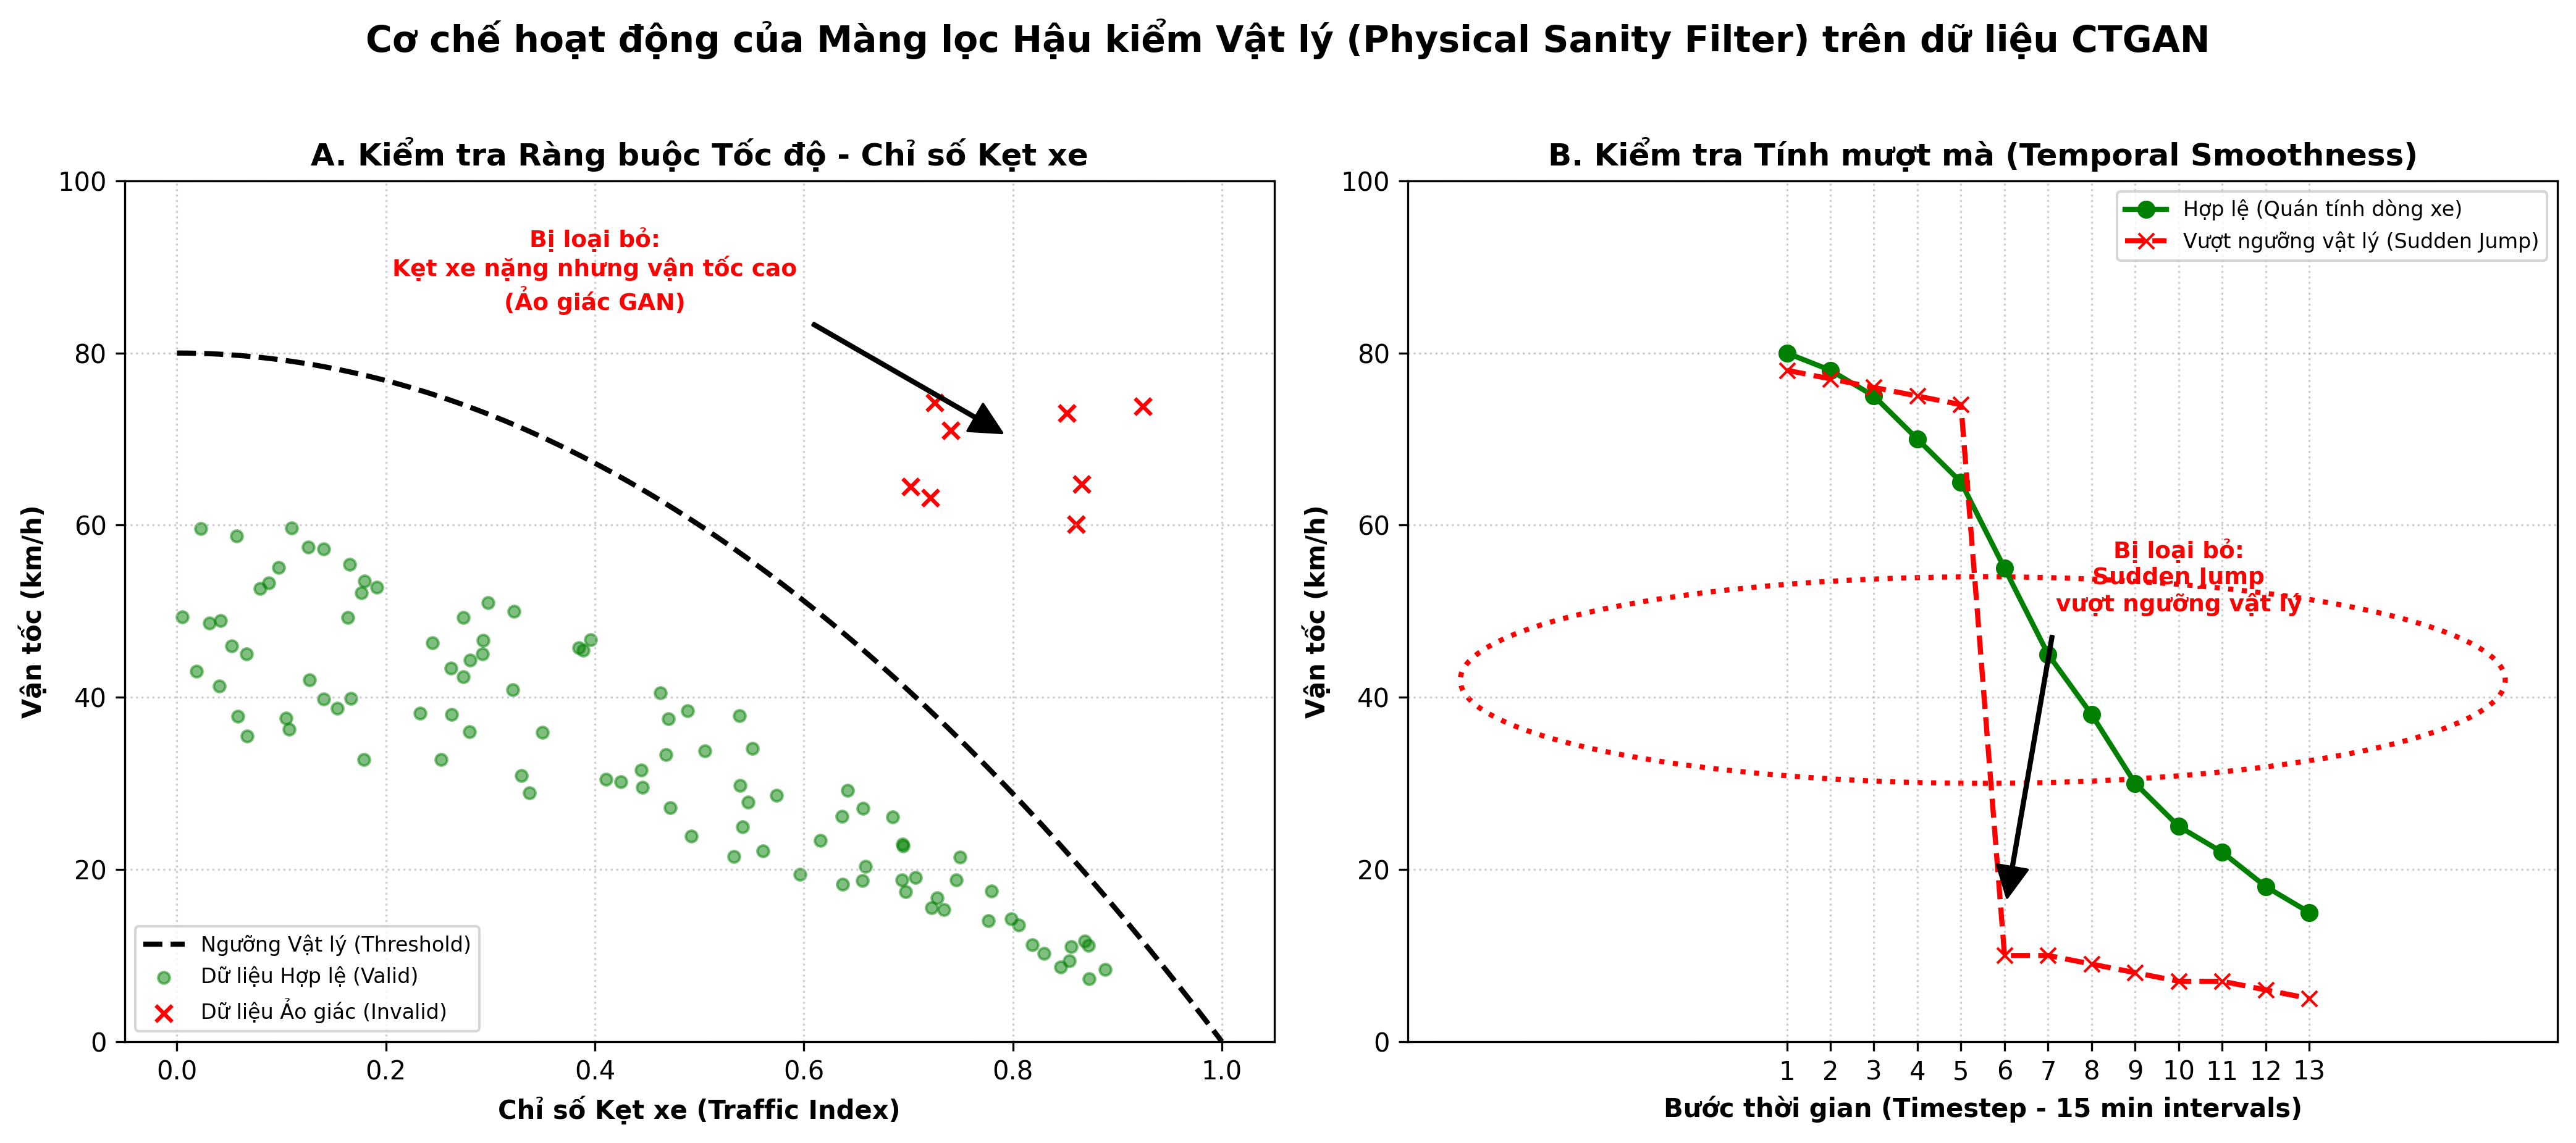
\includegraphics[width=0.8\textwidth]{Images/CH5/14.png}
    \vspace{12pt}
    \caption{Cơ chế hoạt động của Màng lọc Hậu kiểm Vật lý}
    \label{fig:5_14}
\end{figure}

\subsubsection{Xây dựng "Trực giác" ban đầu cho Agent thông qua Học có giám sát (Supervised Pre-training)}

\paragraph{a. Triết lý thiết kế: Khắc phục hội chứng "Khởi động lạnh" (Cold-start Problem)} \mbox{} \\
Trong kiến trúc Học tăng cường thuần túy, mạng Nơ-ron thường khởi tạo các trọng số (weights) một cách ngẫu nhiên. Khi áp dụng vào bài toán giao thông, điều này đồng nghĩa với việc Agent sẽ bắt đầu ở trạng thái "hoàn toàn mù mờ" về các định luật vật lý cơ bản. Agent sẽ phải tốn hàng ngàn chu kỳ (episodes) thực hiện các hành động ngẫu nhiên chỉ để lờ mờ nhận ra các quy luật đơn giản.

Để phá vỡ rào cản này, đồ án thiết lập một pha \textbf{Tiền huấn luyện Giám sát (Supervised Pre-training)}. Triết lý ở đây là tạo ra một "Người thầy" (Supervised Model) để truyền đạt trực giác vật lý ban đầu cho Agent trên Tập dữ liệu Vàng.

\paragraph{b. Tính đồng nhất về Kiến trúc (Architectural Consistency)} \mbox{} \\
Để tri thức có thể được chuyển giao (Transfer) một cách trọn vẹn, kiến trúc của mô hình tiền huấn luyện được thiết kế \textbf{đồng nhất tuyệt đối} với mạng Q-Network của Agent DQN (bao gồm các luồng LSTM xử lý chuỗi thời gian, các tầng Embedding mã hóa không gian và các tầng Fully Connected). Việc sử dụng chung một khuôn mẫu đảm bảo rằng mọi ma trận trọng số (Weight Matrices) học được có thể được nạp trực tiếp (Inject) vào Agent RL ở giai đoạn sau.

\paragraph{c. Tối ưu hóa hàm mất mát với Focal Loss và Trọng số Phạt (Class Weights)} \mbox{} \\
Ngay cả khi tập dữ liệu đã được cân bằng, ranh giới vật lý giữa các mức độ giao thông thường rất mờ nhạt. Để ép mô hình phải tập trung trí lực vào các thảm họa thực sự, đồ án áp dụng:
\begin{enumerate}
    \item \textbf{Focal Loss:} Thay vì sử dụng Cross-Entropy truyền thống vốn đối xử bình đẳng với mọi mẫu, Focal Loss thêm vào một tham số điều biến $\gamma$. Cơ chế này chủ động hạ thấp trọng số của các mẫu "dễ đoán" (ví dụ: đường vắng lúc 2h sáng), ép mạng Nơ-ron dồn toàn bộ đạo hàm (Gradients) để học các mẫu "khó đoán" và mang tính ranh giới.
    \item \textbf{Ma trận Trọng số Nhãn (Class Weights):} Hệ thống được cấu hình để phân bổ mức phạt (Penalty) tỷ lệ nghịch với độ an toàn của trạng thái. Các lớp thảm họa (4 và 5) phải chịu trọng số phạt cực nặng (lên tới $1.8$) so với các lớp an toàn ($0.8$).
\end{enumerate}

\begin{figure}[H]
    \centering
    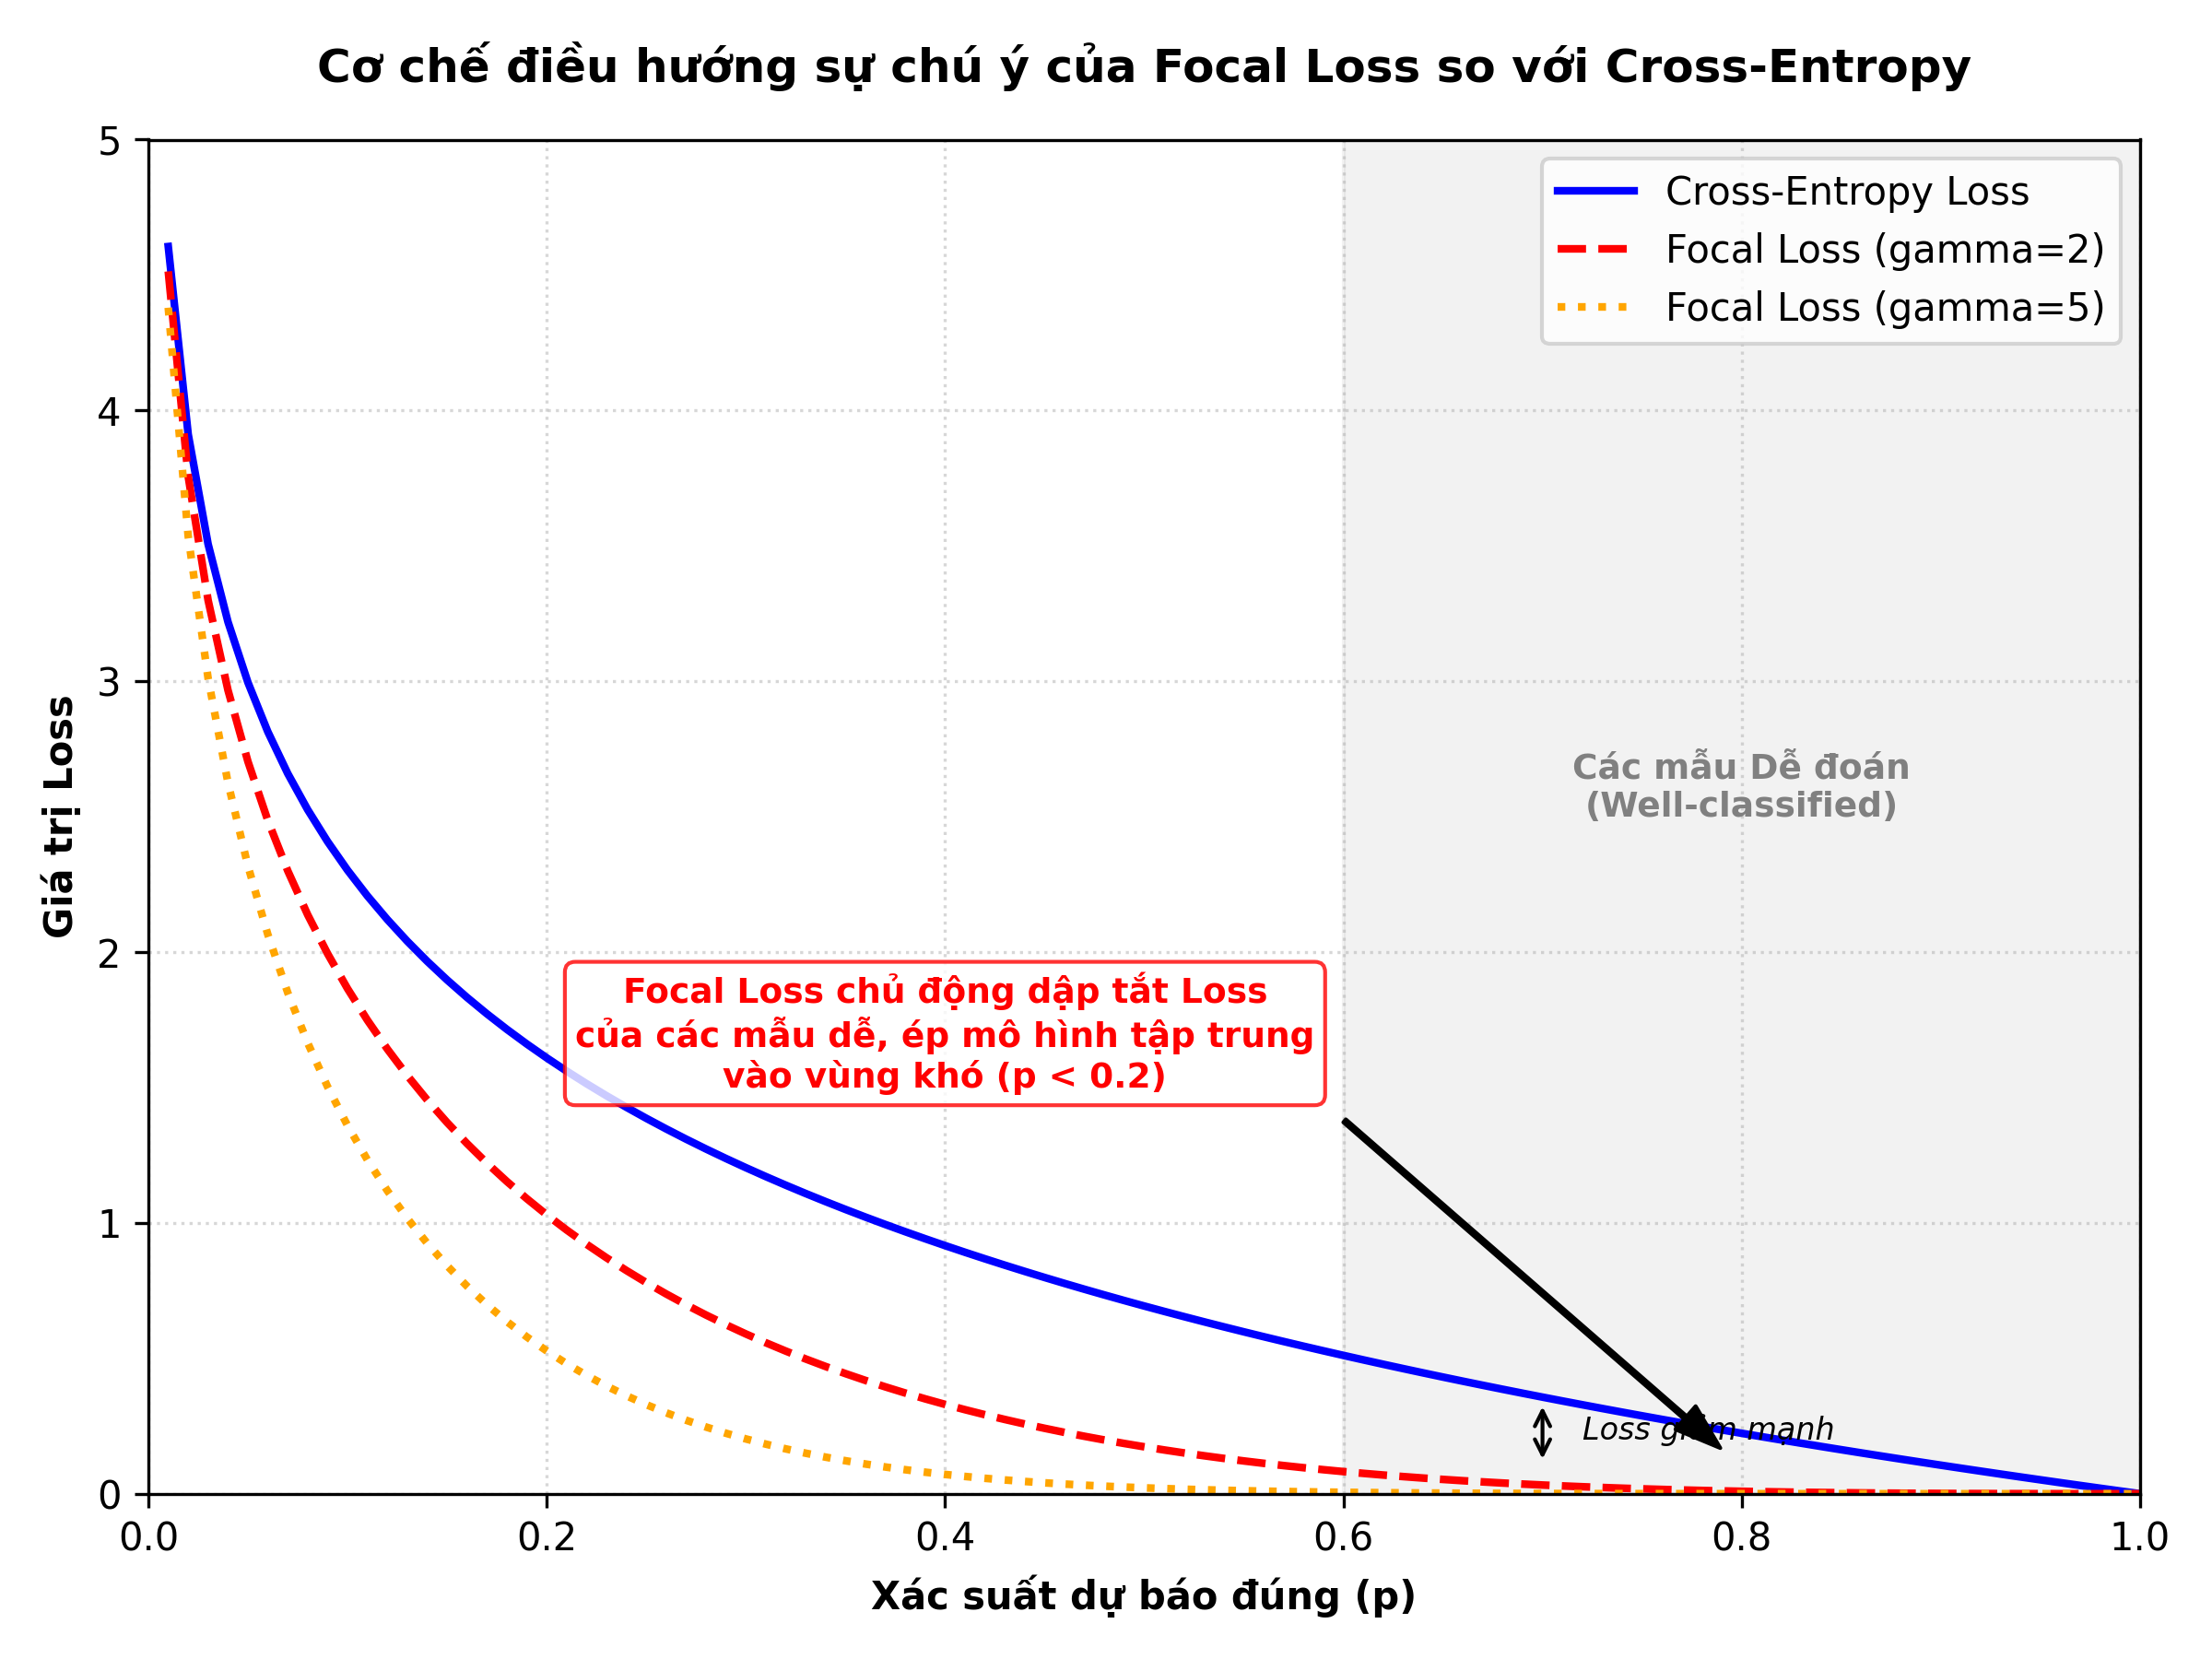
\includegraphics[width=0.8\textwidth]{Images/CH5/15.png}
    \vspace{12pt}
    \caption{Cơ chế điều hướng sự chú ý của Focal Loss so với Cross-Entropy}
    \label{fig:5_15}
\end{figure}

\paragraph{d. Đánh giá Hiệu suất Tiền huấn luyện (Pre-training Performance)} \mbox{} \\
Kết quả thực nghiệm ghi nhận mô hình đạt đỉnh hội tụ ở chỉ số \textbf{Macro-F1 xấp xỉ 0.7}. Điểm nhấn thực sự nằm ở năng lực Thu hồi (Recall): Mô hình đã phát triển một "khứu giác" nhạy bén, khả năng bắt trúng các thảm họa Lớp 4 và Lớp 5 đạt mức tiệm cận $83\% - 84\%$. Bộ trọng số này chính thức hoàn thành nhiệm vụ xây dựng trực giác ban đầu, sẵn sàng để được cấy ghép vào "não bộ" của Agent Học tăng cường.

\begin{figure}[H]
    \centering
    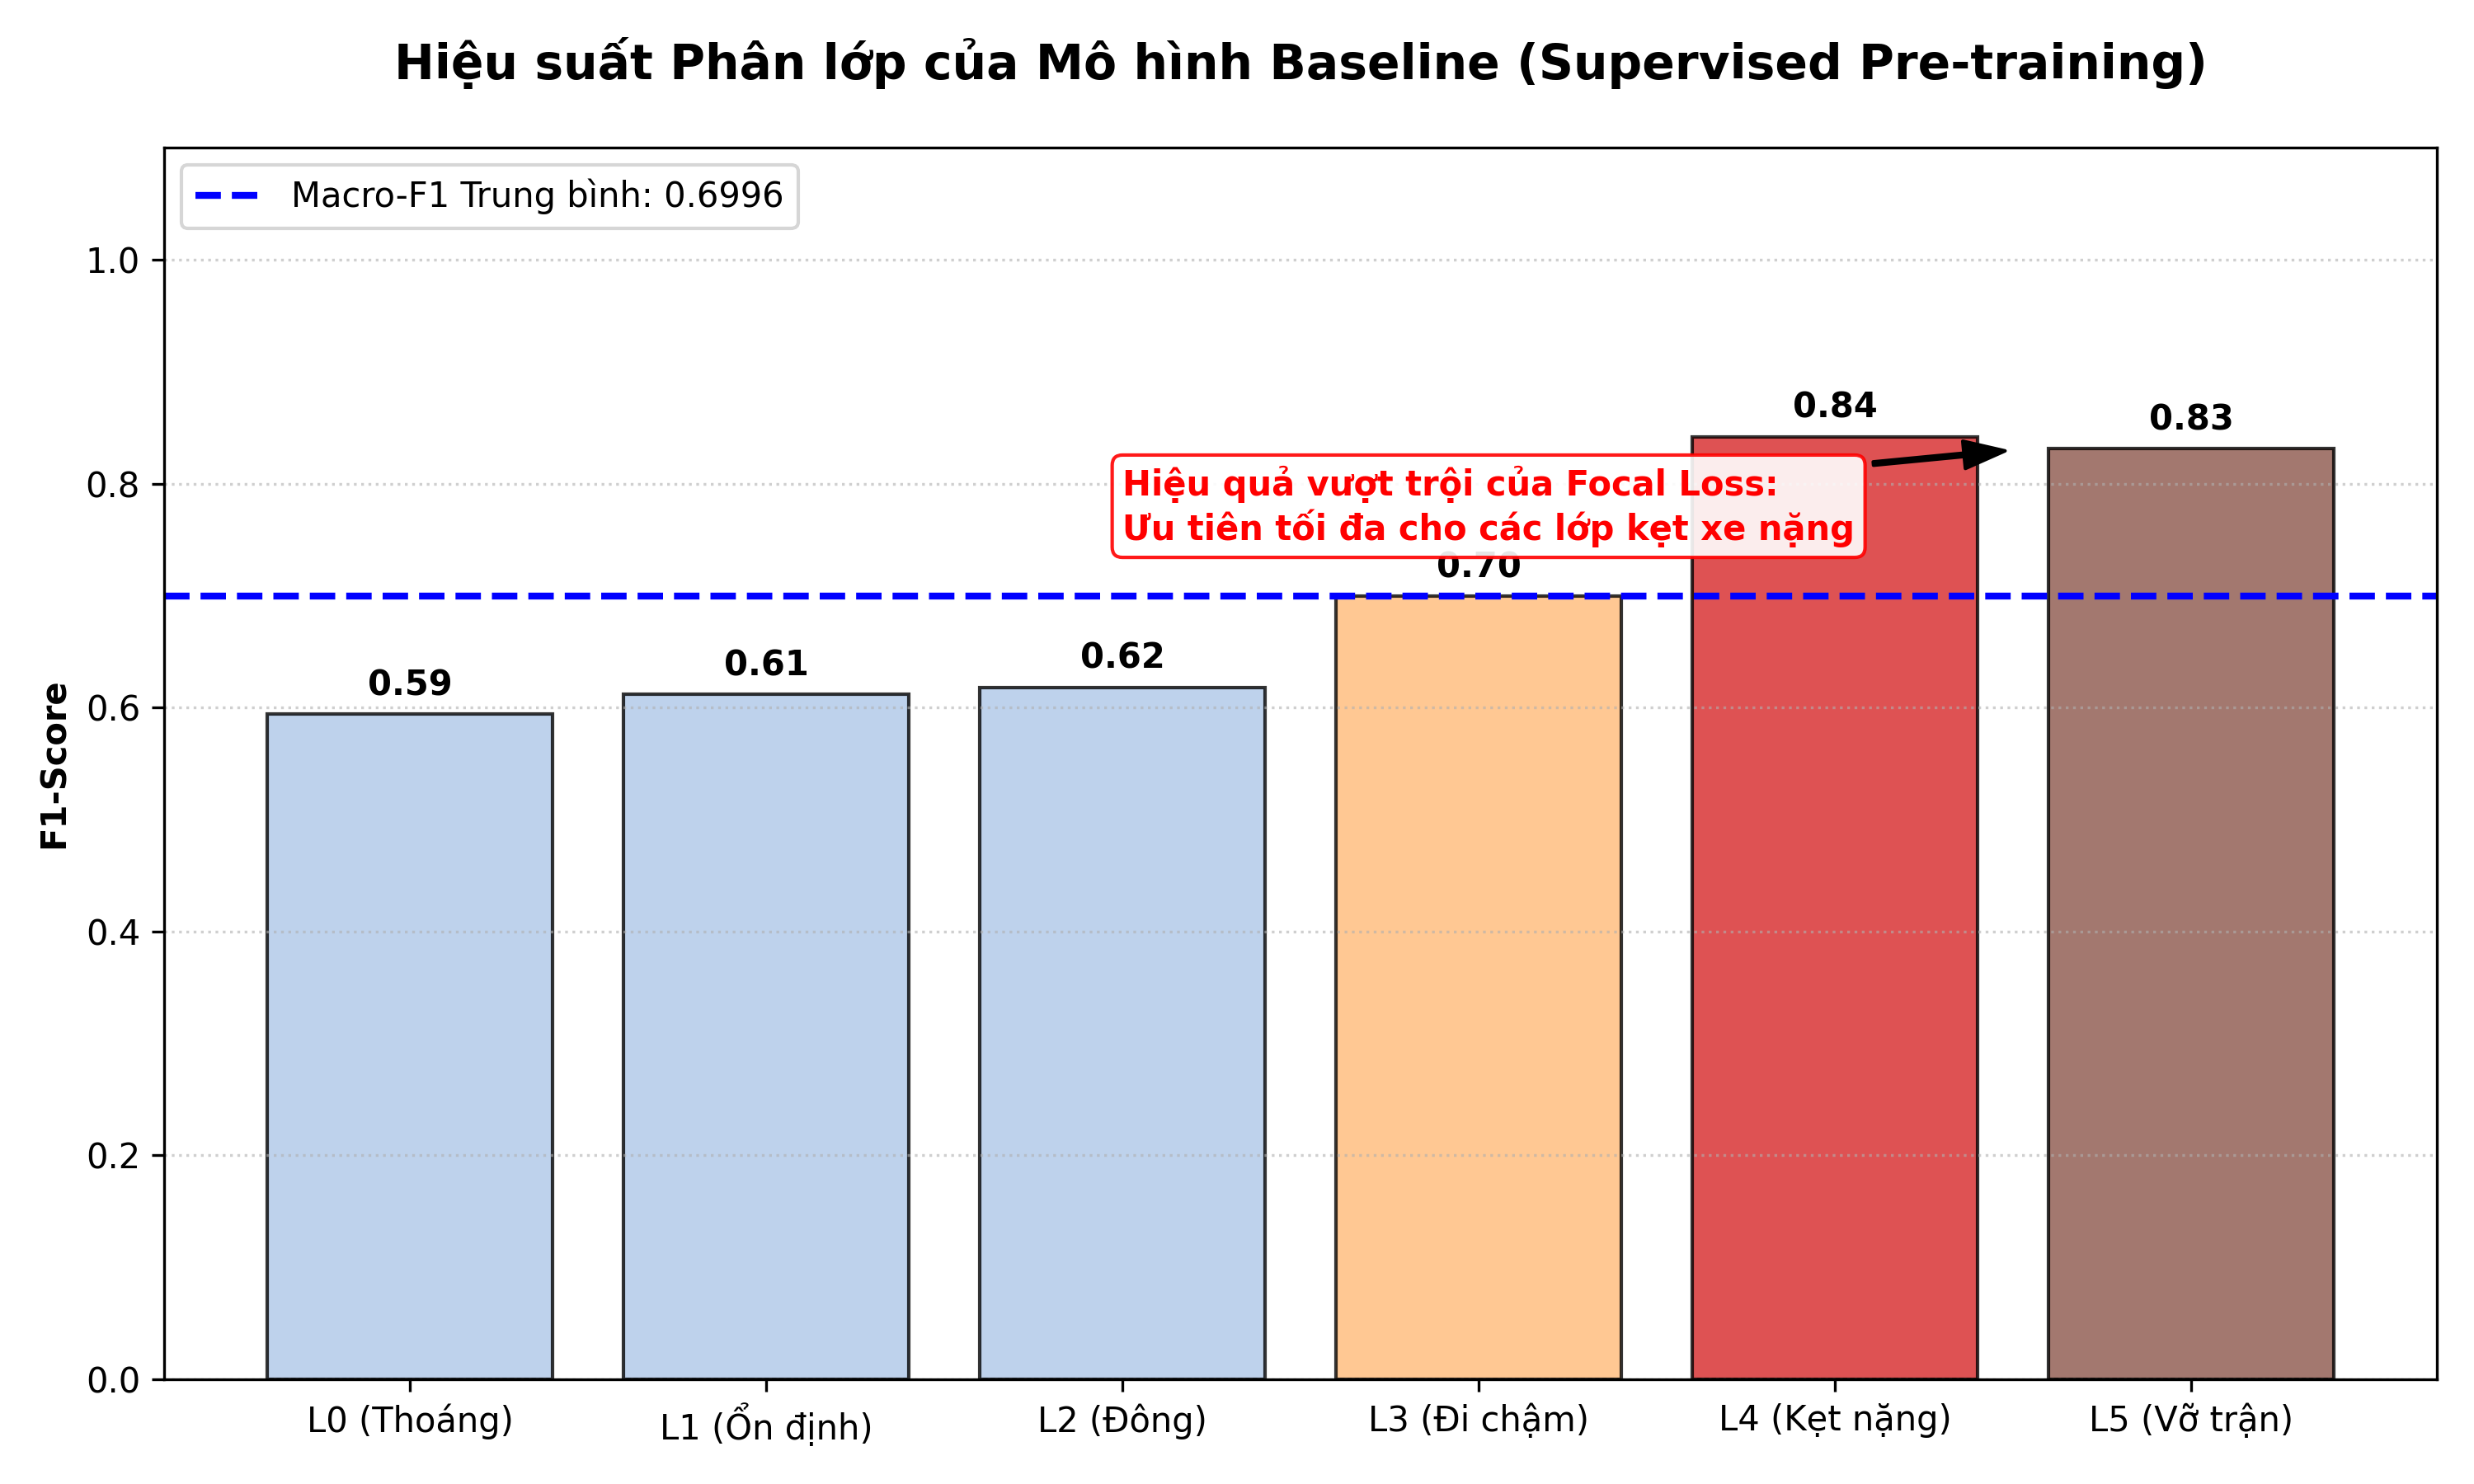
\includegraphics[width=0.8\textwidth]{Images/CH5/16.png}
    \vspace{12pt}
    \caption{Đánh giá hiệu suất Phân lớp của Mô hình Baseline}
    \label{fig:5_16}
\end{figure}

\subsubsection{Giải pháp khắc phục vấn đề "Khởi động lạnh" (Cold Start) trong Học tăng cường}

\paragraph{a. Thách thức từ sự thám hiểm ngẫu nhiên (Random Exploration Dilemma)} \mbox{} \\
Trong một quy trình RL tiêu chuẩn, mạng Q-Network ban đầu được khởi tạo với các trọng số hoàn toàn ngẫu nhiên. Do Agent chưa có bất kỳ khái niệm nào về bối cảnh không gian hay động lực học dòng xe, nó sẽ đưa ra hàng ngàn quyết định vô nghĩa và phi vật lý. Hậu quả là:
\begin{enumerate}
    \item \textbf{Đầu độc bộ nhớ:} Replay Buffer nhanh chóng bị lấp đầy bởi các bước chuyển trạng thái rác.
    \item \textbf{Lãng phí tài nguyên:} Hệ thống phải đốt cháy một lượng khổng lồ tài nguyên tính toán qua hàng vạn chu kỳ chỉ để Agent nhận ra những quy luật đơn giản nhất.
\end{enumerate}

\paragraph{b. Cơ chế "Tiêm tri thức" (Knowledge Injection \& Weight Transfer)} \mbox{} \\
Để khắc phục, đồ án áp dụng cơ chế \textbf{"Khởi động ấm" (Warm-start)} bằng cách "tiêm" trực tiếp tri thức từ Trạm tiền huấn luyện giám sát vào mạng nơ-ron của Agent:
\begin{itemize}
    \item Toàn bộ ma trận trọng số và hệ số chệch được sao chép chính xác (1:1) vào cả hai mạng của kiến trúc Double DQN: \textbf{Policy Network} (Mạng quyết định) và \textbf{Target Network} (Mạng mục tiêu).
    \item Nhờ đó, ngay tại chu kỳ đầu tiên, Agent đã có năng lực nhận diện bối cảnh sắc bén của một chuyên gia giám sát, và chỉ dùng sức mạnh của RL để tinh chỉnh (fine-tune) lại quyết định nhằm tối ưu hóa Hàm phần thưởng không đối xứng.
\end{itemize}

\paragraph{c. Đóng gói và Đồng bộ hóa Hệ sinh thái (MLOps Artifacts Synchronization)} \mbox{} \\
Để đảm bảo tính toàn vẹn, đồ án đóng gói toàn bộ hệ sinh thái tri thức thành các tệp Artifacts:
\begin{enumerate}
    \item Tệp \texttt{best\_traffic\_model\_baseline.pt}: Chứa tri thức toán học (Trọng số Nơ-ron).
    \item Tệp \texttt{preprocessing\_artifacts.pkl}: Chứa hệ quy chiếu vật lý (Scaler, Label Encoders).
\end{enumerate}
Cơ chế này tạo ra một pipeline kín kẽ, triệt tiêu mọi khả năng rò rỉ hoặc sai lệch dữ liệu, đảm bảo Agent phát huy $100\%$ công lực ngay từ giây phút khởi chạy đầu tiên.

\subsubsection{Chuyển giao trọng số và Khởi động ấm (Warm-start Weight Injection)}

Sự khác biệt cốt lõi giữa Học có giám sát (SL) và Học tăng cường (RL) nằm ở mục tiêu tối ưu. Mô hình SL tối ưu hóa dự báo dựa trên một nhãn có sẵn, trong khi Đặc vụ RL tối ưu hóa chuỗi hành động để đạt được tổng phần thưởng lớn nhất.

\paragraph{a. Cơ chế thực thi kỹ thuật (State-Dict Injection)} \mbox{} \\
Khi Môi trường RL và Agent Double DQN được khởi tạo, hệ thống tiến hành một thủ thuật can thiệp sâu vào cấu trúc PyTorch:
\begin{enumerate}
    \item \textbf{Khóa đồng nhất kiến trúc:} Mạng Q-Network được định nghĩa với kiến trúc giống hệt mạng phân lớp đa nhánh (LSTM + Embedding + FNN) đã trình bày.
    \item \textbf{Load State Dict:} Hệ thống gọi trực tiếp từ điển trạng thái (State Dictionary) từ tệp \texttt{best\_traffic\_model\_manual\_h15.pt} và ánh xạ tỷ lệ 1:1 sang mạng Q-Network.
\end{enumerate}
Quá trình này giúp Agent rút ngắn tiến trình Thám hiểm (Exploration Bypass), ngay lập tức nhận diện và phân loại chính xác các trạng thái giao thông cơ bản, dành toàn bộ sức mạnh tính toán để học cách tinh chỉnh các trọng số ở những điểm ranh giới để né tránh các mức phạt sinh tử.
